\chapter{Técnicas de integración}

\section{Ejercicios}

\begin{prob} Calcule las siguientes integrales indefinidas
\begin{multicols}{2}
\begin{enumerate}
\item $\displaystyle\int \sqrt{1-4y}\ dy.$
\item $\displaystyle\int x^4\sqrt{3x^5-5}\ dx.$
\item $\displaystyle\int y^2\sec^2(y^3)\ dy.$
\item $\displaystyle\int \dfrac{\left( x^2-4x+6\right)}{x^3-6x^2+18x}\ dx.$
\item $\displaystyle\int x^2 e^x \cos x\,dx.$
\item $\displaystyle\int \dfrac{x^2+2x}{\sqrt{x^3+3x^2+1}}\ dx.$
\item $\displaystyle\int \sec x\tan x\cos\left( \sec x \right)\ dx.$
\item $\displaystyle\int x^2e^x\ dx.$
\item $\displaystyle\int \cos^{2} x\ dx.$
\item $\displaystyle\int \dfrac{xe^x}{\left( x+1\right)^2}\ dx.$
\item $\displaystyle\int \sen t\ln\left( \cos t \right)\ dt.$
\item $\displaystyle\int x\sec^2 x\ dx.$
\item $\displaystyle\int x\arctan x\ dx.$
\item $\displaystyle\int e^x\cos x\ dx.$
\item $\displaystyle\int \sqrt{20-8x-x^2}\ dx.$
\item $\displaystyle\int \dfrac{5x-1}{x^2-1}\ dx.$
\item $\displaystyle\int \dfrac{3x-13}{(x+2)(x-5)}\ dx.$
\item $\displaystyle\int \cos x\sqrt{4-\sen^2 x}\ dx.$
\item $\displaystyle\int \dfrac{2x^2+3x+2}{x^3+4x^2+6x+4}\ dx.$
\item $\displaystyle\int \dfrac{1}{9x^4+x^2}\ dx.$
\item $\displaystyle\int \dfrac{e^{5x}}{\left(e^{2x} + 1 \right)^2}\ dx.$
\item $\displaystyle\int \dfrac{\ln x}{x^2}\ dx.$
\item $\displaystyle\int \dfrac{2x^2-x-20}{x^2+x-6}\ dx.$
\item $\displaystyle\int \dfrac{2x^2-5x+1}{x^3-2x^2-x+2}\ dx.$
\item $\displaystyle\int \frac{x^3+2x^2-3x+1}{x^2-1}\,dx.$
\item $\displaystyle\int \frac{x^2}{(x-1)^2(x^2+4)}\,dx.$
\item $\displaystyle\int \frac{2x^3-5x^2+4x-1}{(x^2+1)^2}\,dx.$
\item $\displaystyle\int \frac{x^2\ln x}{x^2+1}\,dx.$
\end{enumerate}
\end{multicols}
\end{prob}





La integración, en su formulación más elemental, puede entenderse como la operación inversa de la diferenciación. Sin embargo, mientras que toda función elemental diferenciable produce una derivada elemental, la situación inversa es radicalmente distinta: existen funciones perfectamente continuas y bien comportadas cuya primitiva no puede expresarse en términos de funciones elementales. Esta asimetría profunda entre diferenciación e integración motivó el desarrollo histórico de un amplio arsenal de técnicas de transformación algebraica y trigonométrica que permiten reducir integrales complejas a formas conocidas.

Entre las técnicas más elegantes de este arsenal se encuentran la \textbf{integración de potencias trigonométricas} y la \textbf{sustitución trigonométrica}. La primera explota la riqueza algebraica de las identidades pitagóricas para descomponer potencias de funciones trigonométricas en factores más simples. La segunda, notablemente ingeniosa, utiliza la geometría del triángulo rectángulo para eliminar radicales de la forma $\sqrt{a^2 \pm u^2}$ o $\sqrt{u^2 - a^2}$, transformando expresiones irracionales en integrales trigonométricas tratables.

\begin{rem}
La sistematización de estas técnicas se consolidó en los siglos XVIII y XIX, principalmente a través del trabajo de Euler, Lagrange y los desarrollos incluidos en los tratados de Lacroix y posteriormente en los textos modernos de Purcell, Larson y Stewart. Es importante subrayar que en todos los casos la estrategia fundamental es la misma: transformar la integral original en otra cuya forma sea reconocible, sin alterar el valor del resultado.
\end{rem}

\section{Identidades Trigonométricas Esenciales}

Antes de abordar las técnicas de integración, conviene consolidar el catálogo de identidades trigonométricas que las sustentan. Estas identidades no deben memorizarse como fórmulas aisladas, sino comprenderse como consecuencias del teorema de Pitágoras y de las definiciones de las funciones trigonométricas sobre el círculo unitario.

\begin{theorem}[Identidades pitagóricas]
Para todo ángulo $x \in \R$ donde las funciones involucradas estén definidas:
\[
\sin^2 x + \cos^2 x = 1, \qquad 1 + \tan^2 x = \sec^2 x, \qquad \cot^2 x + 1 = \csc^2 x.
\]
\end{theorem}

\begin{theorem}[Identidades de ángulo doble y reducción de potencia]
\[
\sin^2 x = \frac{1 - \cos 2x}{2}, \qquad \cos^2 x = \frac{1 + \cos 2x}{2}, \qquad \sin x \cos x = \frac{\sin 2x}{2}.
\]
\end{theorem}

\begin{theorem}[Fórmulas de producto a suma]
\[
\sin A \cos B = \tfrac{1}{2}[\sin(A+B) + \sin(A-B)],
\]
\[
\sin A \sin B = \tfrac{1}{2}[\cos(A-B) - \cos(A+B)],
\]
\[
\cos A \cos B = \tfrac{1}{2}[\cos(A-B) + \cos(A+B)].
\]
\end{theorem}

\begin{rem}
Las fórmulas de reducción de potencia $\sin^2 x = \frac{1-\cos 2x}{2}$ y $\cos^2 x = \frac{1+\cos 2x}{2}$ son, junto con la identidad $\sin^2 x + \cos^2 x = 1$, las herramientas más utilizadas en la integración de potencias trigonométricas. Su uso sistemático permite reducir cualquier potencia entera de $\sin x$ o $\cos x$ a una combinación lineal de funciones trigonométricas de múltiplos del ángulo.
\end{rem}

\section{Integración de Potencias Trigonométricas}

\subsection{Integrales de la forma $\int \sin^m x \cos^n x \, dx$}

La estrategia para evaluar esta familia de integrales depende de la paridad de los exponentes $m$ y $n$. La idea central en todos los casos es aislar un factor diferencial $du$ compatible con una sustitución algebraica, y luego convertir el integrando restante a la nueva variable.

\begin{pasos}
\textbf{Caso 1: $m$ impar.} Se escribe $\sin^m x = \sin^{m-1} x \cdot \sin x$ y se reserva el factor $\sin x \, dx$ como el diferencial de la sustitución $u = \cos x$ (pues $du = -\sin x \, dx$). El factor $\sin^{m-1} x$, cuya potencia es ahora par, se convierte completamente a cosenos mediante la identidad $\sin^2 x = 1 - \cos^2 x$.

\textbf{Caso 2: $n$ impar.} Se escribe $\cos^n x = \cos^{n-1} x \cdot \cos x$ y se reserva $\cos x \, dx$ para la sustitución $u = \sin x$ (pues $du = \cos x \, dx$). El factor $\cos^{n-1} x$ se convierte a senos mediante $\cos^2 x = 1 - \sin^2 x$.

\textbf{Caso 3: $m$ y $n$ ambos pares.} No existe un factor diferencial natural para sustitución algebraica. Se aplican las identidades de reducción de potencia para disminuir los exponentes, posiblemente de forma iterativa, hasta obtener integrales de senos y cosenos de ángulos múltiples, que se integran directamente.
\end{pasos}

\begin{example}
Calcular $\displaystyle\int \sin^3 x \cos^2 x \, dx$.
\end{example}

\begin{myproof}
El exponente de $\sin x$ es impar ($m = 3$), así que aplicamos el Caso 1. Separamos:
\[
\int \sin^3 x \cos^2 x \, dx = \int \sin^2 x \cos^2 x \cdot \sin x \, dx.
\]
Sustituimos $u = \cos x$, $du = -\sin x \, dx$, y reemplazamos $\sin^2 x = 1 - \cos^2 x = 1 - u^2$:
\[
= -\int (1 - u^2)\, u^2 \, du = -\int (u^2 - u^4)\, du = -\frac{u^3}{3} + \frac{u^5}{5} + C.
\]
Volviendo a la variable original:
\[
\int \sin^3 x \cos^2 x \, dx = -\frac{\cos^3 x}{3} + \frac{\cos^5 x}{5} + C. \qquad \square
\]
\end{myproof}

\begin{example}
Calcular $\displaystyle\int \sin^2 x \cos^2 x \, dx$.
\end{example}

\begin{myproof}
Ambos exponentes son pares ($m = n = 2$). Aplicamos el Caso 3. Usamos $\sin x \cos x = \frac{\sin 2x}{2}$, de modo que:
\[
\sin^2 x \cos^2 x = \left(\frac{\sin 2x}{2}\right)^2 = \frac{\sin^2 2x}{4} = \frac{1 - \cos 4x}{8}.
\]
Por tanto:
\[
\int \sin^2 x \cos^2 x \, dx = \int \frac{1 - \cos 4x}{8}\, dx = \frac{x}{8} - \frac{\sin 4x}{32} + C. \qquad \square
\]
\end{myproof}

\begin{theorem}[Fórmula de reducción para $\sin^n x$]
\[
\int \sin^n x \, dx = -\frac{\sin^{n-1} x \cos x}{n} + \frac{n-1}{n} \int \sin^{n-2} x \, dx.
\]
\end{theorem}

\begin{theorem}[Fórmula de reducción para $\cos^n x$]
\[
\int \cos^n x \, dx = \frac{\cos^{n-1} x \sin x}{n} + \frac{n-1}{n} \int \cos^{n-2} x \, dx.
\]
\end{theorem}

\begin{rem}
Las fórmulas de reducción permiten calcular $\int \sin^n x \, dx$ o $\int \cos^n x \, dx$ para cualquier entero $n \geq 2$, reduciendo iterativamente el exponente hasta llegar a $\int \sin x \, dx = -\cos x + C$ (si $n$ es impar) o a $\int dx = x + C$ (si $n$ es par, tras la reducción final). Estas fórmulas se demuestran por integración por partes.
\end{rem}

\subsection{Integrales de la forma $\int \tan^m x \sec^n x \, dx$}

El tratamiento de estas integrales es análogo al caso anterior, pero usando el par de identidades $1 + \tan^2 x = \sec^2 x$ y la relación diferencial $\frac{d}{dx}(\sec x) = \sec x \tan x$, $\frac{d}{dx}(\tan x) = \sec^2 x$.

\begin{pasos}
\textbf{Caso 1: $n$ par.} Se reserva el factor $\sec^2 x \, dx$ como diferencial de $u = \tan x$ (pues $du = \sec^2 x \, dx$). El factor restante $\sec^{n-2} x$ se convierte a tangentes mediante $\sec^2 x = 1 + \tan^2 x$.

\textbf{Caso 2: $m$ impar.} Se reserva el factor $\sec x \tan x \, dx$ como diferencial de $u = \sec x$ (pues $du = \sec x \tan x \, dx$). El factor restante $\tan^{m-1} x$ se convierte a secantes mediante $\tan^2 x = \sec^2 x - 1$.

\textbf{Caso 3: $m$ par y $n$ impar.} No existe sustitución directa conveniente. Se convierte todo a secantes usando $\tan^2 x = \sec^2 x - 1$, y se recurre a fórmulas de reducción o integración por partes.
\end{pasos}

\begin{example}
Calcular $\displaystyle\int \tan^3 x \sec^4 x \, dx$.
\end{example}

\begin{myproof}
El exponente de $\sec x$ es par ($n=4$), así que aplicamos el Caso 1. Reservamos $\sec^2 x\,dx$ y convertimos el resto:
\[
\int \tan^3 x \sec^4 x\, dx = \int \tan^3 x \sec^2 x \cdot \sec^2 x\, dx = \int \tan^3 x (1 + \tan^2 x)\sec^2 x\, dx.
\]
Con $u = \tan x$, $du = \sec^2 x\, dx$:
\[
= \int u^3(1 + u^2)\, du = \int (u^3 + u^5)\, du = \frac{u^4}{4} + \frac{u^6}{6} + C = \frac{\tan^4 x}{4} + \frac{\tan^6 x}{6} + C. \qquad \square
\]
\end{myproof}

\subsection{Integrales de productos cruzados: $\int \sin(mx)\cos(nx)\, dx$}

Cuando el integrando es un producto de seno y coseno de distintos ángulos, ninguna de las estrategias anteriores aplica directamente. En este caso se utilizan las fórmulas de producto a suma para convertir el producto en una suma de funciones trigonométricas simples, que se integran directamente término a término.

\begin{example}
Calcular $\displaystyle\int \sin(3x)\cos(5x)\, dx$.
\end{example}

\begin{myproof}
Aplicamos la fórmula $\sin A \cos B = \frac{1}{2}[\sin(A+B) + \sin(A-B)]$ con $A = 3x$, $B = 5x$:
\[
\sin(3x)\cos(5x) = \tfrac{1}{2}[\sin(8x) + \sin(-2x)] = \tfrac{1}{2}[\sin(8x) - \sin(2x)].
\]
Integrando:
\[
\int \sin(3x)\cos(5x)\, dx = \frac{1}{2}\left[-\frac{\cos 8x}{8} + \frac{\cos 2x}{2}\right] + C = -\frac{\cos 8x}{16} + \frac{\cos 2x}{4} + C. \qquad \square
\]
\end{myproof}

\section{Sustitución Trigonométrica}

\subsection{Idea Geométrica y Fundamento}

La sustitución trigonométrica es una técnica que permite eliminar radicales del integrando mediante la introducción de un ángulo $\theta$ como nueva variable de integración. El fundamento geométrico de la técnica reside en las identidades pitagóricas: si se identifica la expresión bajo el radical con uno de los lados de un triángulo rectángulo, la relación entre los lados del triángulo permite simplificar el radical a una función trigonométrica simple.

La técnica opera en tres fases: (1) se elige la sustitución trigonométrica apropiada según la forma del radical; (2) se transforma la integral completa ---incluyendo el diferencial $dx$--- a la variable $\theta$; (3) una vez evaluada la integral en términos de $\theta$, se utiliza el triángulo de referencia para regresar a la variable original $x$.

\begin{rem}
Al usar sustitución trigonométrica en integrales definidas, se puede trabajar de dos maneras equivalentes: transformar los límites de integración a valores de $\theta$ al momento de hacer la sustitución (y no regresar a $x$), o evaluar la antiderivada en términos de $x$ y luego aplicar los límites originales. La primera estrategia es generalmente más eficiente.
\end{rem}

\subsection{Caso 1: Radical $\sqrt{a^2 - u^2}$}

Cuando el integrando contiene $\sqrt{a^2 - u^2}$ con $a > 0$, se utiliza la sustitución $u = a\sin\theta$, con $\theta \in \left[-\frac{\pi}{2}, \frac{\pi}{2}\right]$. Bajo esta sustitución, $du = a\cos\theta\, d\theta$ y:
\[
\sqrt{a^2 - u^2} = \sqrt{a^2 - a^2\sin^2\theta} = a\sqrt{1 - \sin^2\theta} = a\cos\theta,
\]
donde el signo positivo es válido porque $\cos\theta \geq 0$ en el intervalo restringido. El triángulo de referencia asociado tiene hipotenusa $a$, cateto opuesto a $\theta$ igual a $u$, y cateto adyacente $\sqrt{a^2 - u^2}$.

\begin{center}
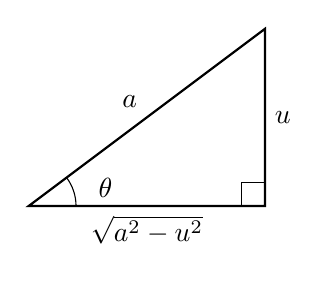
\begin{tikzpicture}[scale=1.5]
    % Triángulo
    \draw[thick] (0,0) -- (2,0) -- (2,1.5) -- cycle;
    % Ángulo recto
    \draw (1.8,0) -- (1.8,0.2) -- (2,0.2);
    % Etiquetas de lados
    \node[below] at (1,0) {$\sqrt{a^2 - u^2}$};
    \node[right] at (2,0.75) {$u$};
    \node[above left] at (1,0.75) {$a$};
    % Ángulo theta
    \draw (0.4,0) arc (0:36.87:0.4);
    \node at (0.65,0.15) {$\theta$};
\end{tikzpicture}
\end{center}

\begin{example}
Calcular $\displaystyle\int \frac{dx}{\sqrt{9 - x^2}}$.
\end{example}

\begin{myproof}
Identificamos $a = 3$ y sustituimos $x = 3\sin\theta$, $dx = 3\cos\theta\, d\theta$:
\[
\sqrt{9 - x^2} = \sqrt{9 - 9\sin^2\theta} = 3\cos\theta.
\]
La integral se transforma en:
\[
\int \frac{3\cos\theta\, d\theta}{3\cos\theta} = \int d\theta = \theta + C = \arcsin\!\left(\frac{x}{3}\right) + C. \qquad \square
\]
\end{myproof}

\begin{example}
Calcular $\displaystyle\int x^2\sqrt{4 - x^2}\, dx$.
\end{example}

\begin{myproof}
Con $a = 2$: $x = 2\sin\theta$, $dx = 2\cos\theta\, d\theta$, $\sqrt{4 - x^2} = 2\cos\theta$. Entonces:
\[
\int (4\sin^2\theta)(2\cos\theta)(2\cos\theta)\, d\theta = 16\int \sin^2\theta\cos^2\theta\, d\theta = 16\int \frac{\sin^2 2\theta}{4}\, d\theta = 4\int \frac{1 - \cos 4\theta}{2}\, d\theta.
\]
\[
= 2\theta - \frac{\sin 4\theta}{2} + C.
\]
Para regresar a $x$: del triángulo, $\theta = \arcsin\!\left(\frac{x}{2}\right)$, $\sin\theta = \frac{x}{2}$, $\cos\theta = \frac{\sqrt{4-x^2}}{2}$. Usando $\sin 4\theta = 2\sin 2\theta\cos 2\theta = 4\sin\theta\cos\theta(1 - 2\sin^2\theta)$:
\[
\int x^2\sqrt{4-x^2}\, dx = 2\arcsin\!\left(\frac{x}{2}\right) - \frac{x(4-x^2)^{1/2}(4 - 2x^2)}{8} + C. \qquad \square
\]
\end{myproof}

\subsection{Caso 2: Radical $\sqrt{a^2 + u^2}$}

Cuando el integrando contiene $\sqrt{a^2 + u^2}$, se usa $u = a\tan\theta$ con $\theta \in \left(-\frac{\pi}{2}, \frac{\pi}{2}\right)$, de modo que $du = a\sec^2\theta\, d\theta$ y:
\[
\sqrt{a^2 + u^2} = \sqrt{a^2 + a^2\tan^2\theta} = a\sqrt{1 + \tan^2\theta} = a\sec\theta.
\]
El triángulo de referencia tiene cateto adyacente $a$, cateto opuesto $u$, e hipotenusa $\sqrt{a^2 + u^2}$.

\begin{center}
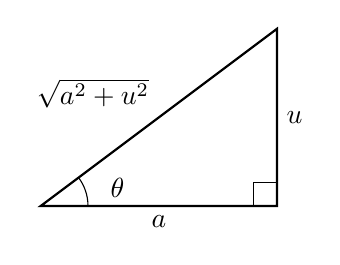
\begin{tikzpicture}[scale=1.5]
    \draw[thick] (0,0) -- (2,0) -- (2,1.5) -- cycle;
    \draw (1.8,0) -- (1.8,0.2) -- (2,0.2);
    \node[below] at (1,0) {$a$};
    \node[right] at (2,0.75) {$u$};
    \node[above left] at (1,0.75) {$\sqrt{a^2 + u^2}$};
    \draw (0.4,0) arc (0:36.87:0.4);
    \node at (0.65,0.15) {$\theta$};
\end{tikzpicture}
\end{center}

\begin{example}
Calcular $\displaystyle\int \frac{dx}{\sqrt{x^2 + 16}}$.
\end{example}

\begin{myproof}
Con $a = 4$: $x = 4\tan\theta$, $dx = 4\sec^2\theta\, d\theta$, $\sqrt{x^2 + 16} = 4\sec\theta$:
\[
\int \frac{4\sec^2\theta\, d\theta}{4\sec\theta} = \int \sec\theta\, d\theta = \ln\abs{\sec\theta + \tan\theta} + C.
\]
Del triángulo: $\tan\theta = \frac{x}{4}$, $\sec\theta = \frac{\sqrt{x^2+16}}{4}$. Entonces:
\[
\int \frac{dx}{\sqrt{x^2+16}} = \ln\left|\frac{\sqrt{x^2+16}}{4} + \frac{x}{4}\right| + C = \ln\abs{\sqrt{x^2+16} + x} + C_1. \qquad \square
\]
\end{myproof}

\subsection{Caso 3: Radical $\sqrt{u^2 - a^2}$}

Cuando el integrando contiene $\sqrt{u^2 - a^2}$, se usa $u = a\sec\theta$ con $\theta \in \left[0, \frac{\pi}{2}\right) \cup \left(\frac{\pi}{2}, \pi\right]$, de modo que $du = a\sec\theta\tan\theta\, d\theta$ y:
\[
\sqrt{u^2 - a^2} = \sqrt{a^2\sec^2\theta - a^2} = a\sqrt{\sec^2\theta - 1} = a\tan\theta.
\]
El triángulo de referencia tiene hipotenusa $u$, cateto adyacente $a$, y cateto opuesto $\sqrt{u^2 - a^2}$.

\begin{center}
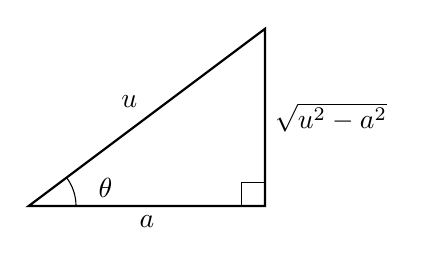
\begin{tikzpicture}[scale=1.5]
    \draw[thick] (0,0) -- (2,0) -- (2,1.5) -- cycle;
    \draw (1.8,0) -- (1.8,0.2) -- (2,0.2);
    \node[below] at (1,0) {$a$};
    \node[right] at (2,0.75) {$\sqrt{u^2 - a^2}$};
    \node[above left] at (1,0.75) {$u$};
    \draw (0.4,0) arc (0:36.87:0.4);
    \node at (0.65,0.15) {$\theta$};
\end{tikzpicture}
\end{center}

\begin{example}
Calcular $\displaystyle\int \frac{\sqrt{x^2 - 9}}{x}\, dx$.
\end{example}

\begin{myproof}
Con $a = 3$: $x = 3\sec\theta$, $dx = 3\sec\theta\tan\theta\, d\theta$, $\sqrt{x^2-9} = 3\tan\theta$:
\[
\int \frac{3\tan\theta \cdot 3\sec\theta\tan\theta\, d\theta}{3\sec\theta} = 3\int \tan^2\theta\, d\theta = 3\int(\sec^2\theta - 1)\, d\theta = 3\tan\theta - 3\theta + C.
\]
Del triángulo: $\tan\theta = \frac{\sqrt{x^2-9}}{3}$, $\theta = \text{arcsec}\!\left(\frac{x}{3}\right)$:
\[
\int \frac{\sqrt{x^2-9}}{x}\, dx = \sqrt{x^2-9} - 3\,\text{arcsec}\!\left(\frac{x}{3}\right) + C. \qquad \square
\]
\end{myproof}

\subsection{Tabla Resumen de Sustituciones}

\begin{center}
\begin{tabular}{>{\bfseries}c c c c}
\toprule
Radical & Sustitución & Diferencial & Simplificación \\
\midrule
$\sqrt{a^2 - u^2}$ & $u = a\sin\theta$ & $du = a\cos\theta\,d\theta$ & $\sqrt{a^2 - u^2} = a\cos\theta$ \\[4pt]
$\sqrt{a^2 + u^2}$ & $u = a\tan\theta$ & $du = a\sec^2\theta\,d\theta$ & $\sqrt{a^2 + u^2} = a\sec\theta$ \\[4pt]
$\sqrt{u^2 - a^2}$ & $u = a\sec\theta$ & $du = a\sec\theta\tan\theta\,d\theta$ & $\sqrt{u^2 - a^2} = a\tan\theta$ \\
\bottomrule
\end{tabular}
\end{center}

\begin{rem}
Cuando el radical involucra una expresión cuadrática general de la forma $\sqrt{ax^2 + bx + c}$, el primer paso siempre es completar el cuadrado para reducirla a una de las tres formas estándar anteriores. Por ejemplo, $\sqrt{x^2 + 4x + 5} = \sqrt{(x+2)^2 + 1}$, que corresponde al Caso 2 con $u = x+2$ y $a = 1$.
\end{rem}

\section{Problemas Propuestos}

\begin{example}
Calcular $\displaystyle \int \sin x \cos x \, dx$.
\end{example}

\begin{myproof}
Usamos la identidad $\sin x \cos x = \dfrac{1}{2}\sin(2x)$. Entonces
\[
\int \sin x \cos x \, dx = \int \frac{1}{2}\sin(2x)\, dx = -\frac{1}{4}\cos(2x) + C.
\]
Alternativamente, podemos usar sustitución. Sea $u = \sin x$, de modo que $du = \cos x\, dx$. Entonces
\[
\int \sin x \cos x \, dx = \int u\, du = \frac{u^2}{2} + C = \frac{\sin^2 x}{2} + C.
\]
Las dos expresiones difieren sólo en una constante aditiva, así que ambas son primitivas válidas. \qquad $\square$
\end{myproof}



\begin{example}
Calcular $\displaystyle \int \frac{dx}{\sqrt{9 - x^2}}$.
\end{example}

\begin{myproof}
La presencia de $\sqrt{9 - x^2}$ sugiere una sustitución trigonométrica del tipo $x = a\sin\theta$ con $a = 3$. Tomamos
\[
x = 3\sin\theta, \qquad dx = 3\cos\theta\, d\theta.
\]
Entonces
\[
\sqrt{9 - x^2} = \sqrt{9 - 9\sin^2\theta} = 3\sqrt{1 - \sin^2\theta} = 3\cos\theta,
\]
donde usamos la identidad pitagórica. Sustituyendo en la integral:
\[
\int \frac{dx}{\sqrt{9 - x^2}} = \int \frac{3\cos\theta\, d\theta}{3\cos\theta} = \int d\theta = \theta + C.
\]
Para regresar a la variable $x$, observamos que $x = 3\sin\theta$ implica $\theta = \arcsin\!\left(\dfrac{x}{3}\right)$. Por lo tanto,
\[
\int \frac{dx}{\sqrt{9 - x^2}} = \arcsin\!\left(\frac{x}{3}\right) + C. \qquad \square
\]
\end{myproof}



\begin{example}
Calcular $\displaystyle \int \sec^5 x \, dx$.
\end{example}

\begin{myproof}
Escribimos $\sec^5 x = \sec^3 x\, \sec^2 x$ y usamos la identidad $\sec^2 x = 1 + \tan^2 x$ junto con una integración por partes clásica. Primero, reescribimos:
\[
\int \sec^5 x\, dx = \int \sec^3 x \sec^2 x\, dx.
\]
Recordemos que $\sec^3 x$ admite la descomposición $\sec^3 x = \sec x (\sec^2 x) = \sec x(1 + \tan^2 x)$. Una estrategia estándar consiste en separar la integral como
\[
\int \sec^5 x\, dx = \int \sec^3 x \sec^2 x\, dx = \int \sec^3 x (1 + \tan^2 x)\, dx,
\]
y realizar integración por partes con
\[
u = \sec^3 x, \qquad dv = \sec^2 x\, dx.
\]
Entonces
\[
du = 3\sec^2 x \sec x \tan x\, dx \quad \text{y} \quad v = \tan x.
\]
Aplicando integración por partes:
\[
\int \sec^5 x\, dx = \sec^3 x \tan x - \int \tan x \cdot 3\sec^2 x \sec x \tan x\, dx
= \sec^3 x \tan x - 3\int \sec^3 x \sec^2 x \tan^2 x\, dx.
\]
Usando $\tan^2 x = \sec^2 x - 1$:
\[
\int \sec^5 x\, dx = \sec^3 x \tan x - 3\int \sec^3 x \sec^2 x(\sec^2 x - 1)\, dx
= \sec^3 x \tan x - 3\int \sec^5 x \sec^2 x\, dx + 3\int \sec^3 x \sec^2 x\, dx.
\]
Es más eficiente proceder con el enfoque clásico: separar un factor $\sec x \tan x$ y usar sustitución. Escribimos
\[
\sec^5 x = \sec^3 x \sec^2 x = \sec^3 x (1 + \tan^2 x)
= \sec^3 x + \sec^3 x \tan^2 x.
\]
Trabajamos con la forma estándar siguiente (resultado conocido que puede comprobarse por integración por partes cuidada):
\[
\int \sec^5 x\, dx = \frac{\sec^3 x \tan x}{4} + \frac{3}{4}\int \sec^3 x\, dx.
\]
La integral de $\sec^3 x$ también es clásica:
\[
\int \sec^3 x\, dx = \frac{1}{2}\sec x \tan x + \frac{1}{2}\ln\abs{\sec x + \tan x} + C.
\]
Sustituyendo este resultado:
\[
\int \sec^5 x\, dx = \frac{\sec^3 x \tan x}{4} + \frac{3}{4}\left[\frac{1}{2}\sec x \tan x + \frac{1}{2}\ln\abs{\sec x + \tan x}\right] + C.
\]
Es decir,
\[
\boxed{\int \sec^5 x\, dx = \frac{\sec^3 x \tan x}{4} + \frac{3}{8}\sec x \tan x + \frac{3}{8}\ln\abs{\sec x + \tan x} + C.}
\]
Cualquier forma algebraicamente equivalente de esta expresión se considera respuesta correcta. \qquad \square
\end{myproof}





\begin{prob}
$\displaystyle \int \sin^3 x \cos^2 x \, dx$
\end{prob}

\begin{prob}
$\displaystyle \int \sec^4(5x) \, dx$
\end{prob}

\begin{prob}
$\displaystyle \int \tan^2 x \, dx$
\end{prob}

\begin{prob}
$\displaystyle \int \frac{dx}{\sqrt{9 - x^2}}$
\end{prob}

\begin{prob}
$\displaystyle \int \sec(7x) \, dx$
\end{prob}

\begin{prob}
$\displaystyle \int \sin x \cos x \, dx$
\end{prob}

\begin{prob}
$\displaystyle \int \frac{dx}{x^2 + 4}$
\end{prob}

\begin{prob}
$\displaystyle \int \sqrt{1 - 4x^2}\, dx$
\end{prob}

 

\begin{prob}
$\displaystyle \int \sin^4(6x)\, dx$
\end{prob}

\begin{prob}
$\displaystyle \int \tan^3\!\left(\frac{x}{2}\right)\sec^2\!\left(\frac{x}{2}\right)\, dx$
\end{prob}

\begin{prob}
$\displaystyle \int \frac{\tan^3 x}{\sqrt{\sec x}} \, dx$
\end{prob}

\begin{prob}
$\displaystyle \int \frac{x^2}{\sqrt{16 - x^2}} \, dx$
\end{prob}

\begin{prob}
$\displaystyle \int \frac{dx}{\sqrt{x^2 - 7}}$
\end{prob}

\begin{prob}
$\displaystyle \int \frac{dt}{t^2\sqrt{t^2 - 16}}$
\end{prob}

\begin{prob}
$\displaystyle \int \tan^3(2x)\sec(2x)\, dx$
\end{prob}

\begin{prob}
$\displaystyle \int \frac{dx}{(x^2 + 4)^{3/2}}$
\end{prob}

\begin{prob}
$\displaystyle \int \sin^3 x \cos^4 x \, dx$
\end{prob}

\begin{prob}
$\displaystyle \int \sqrt{a^2 - x^2}\, dx$
\end{prob}

 

\begin{prob}
$\displaystyle \int \sec^5 x \, dx$
\end{prob}

\begin{prob}
$\displaystyle \int \frac{x^2}{\sqrt{2x - x^2}} \, dx$
\end{prob}

\begin{prob}
$\displaystyle \int \frac{x}{\sqrt{x^2 + 6x + 12}} \, dx$
\end{prob}

\begin{prob}
$\displaystyle \int \sin^4 x \cos^2 x \, dx$
\end{prob}

\begin{prob}
$\displaystyle \int \frac{dx}{x\sqrt{4x^2 + 9}}$
\end{prob}

\begin{prob}
$\displaystyle \int \tan^2 x \sec^5 x \, dx$
\end{prob}

\begin{prob}
$\displaystyle \int \frac{\cos x}{\sqrt{1 + \sin^2 x}} \, dx$
\end{prob}

\begin{prob}
$\displaystyle \int \sqrt{x^2 + 2x}\, dx$
\end{prob}

\begin{prob}
$\displaystyle \int \frac{dz}{z \sqrt{25 - 4z^2}}$
\end{prob}

\begin{prob}
$\displaystyle \int \frac{x^2}{\sqrt{5 - 4x^2}} \, dx$
\end{prob}

\begin{prob}
$\displaystyle \int \sqrt{\tan x} \, dx$  
\end{prob}

\begin{prob}
$\displaystyle \int \frac{dx}{x^6 + 1}$  
\end{prob}

\begin{prob}
$\displaystyle \int \frac{dx}{1 + \sin^2 x}$  
\end{prob}

\begin{prob}
$\displaystyle \int \sec^5 x \, dx$  
\end{prob}

\begin{prob}
$\displaystyle \int \frac{dx}{x \sqrt{x^n + 1}}$  
\end{prob}

\begin{prob}
$\displaystyle \int \frac{x^2}{(2x - x^2)^{3/2}} \, dx$  
\end{prob}

\begin{prob}
$\displaystyle \int \frac{dx}{x^4 \sqrt{x^2 - 9}}$  
\end{prob}

\begin{prob}
$\displaystyle \int \frac{\cos x}{\sqrt{1 + \sin^2 x}} \, dx$  
\end{prob}

\begin{prob}
$\displaystyle \int \frac{dx}{2 - \sin x}$  
\end{prob}

\begin{prob}
$\displaystyle \int_{0}^{\pi/2} \sin^n x \, dx$  
\end{prob}
 

\begin{prob}
$\displaystyle \int \sin^2(5x)\, dx$
\end{prob}

\begin{prob}
$\displaystyle \int \cos^3 x \, dx$
\end{prob}





